% Sprinkler pumpe system

\subsection{Sprinkler-pumpe system ()}

Sprinkleren skal forsynes med et vandtryk fra en vandpumpe. Grundfos har doneret en Alpha2 pumpe til formålet. Alpha2 pumpen kræver 230 VAC. Det overskrider hvad der dagligt må arbejde med for studerende på AU. Der er derfor efter aftale med Torben Lund Jensen fra værkstedet givet særskilt tilladelse til at designe og implementere et lukket 230 V / 5 V relæ. Figur \ref{lab:Relay_box} viser kredsløbet for det lukkede 230 V / 5 V relæ. Jordforbindelsen løber direkte igennem og er altid forbundet, mens fasen og nul forbindes/afbrydes af relæet.  

\begin{figure}[H]
  \centering
    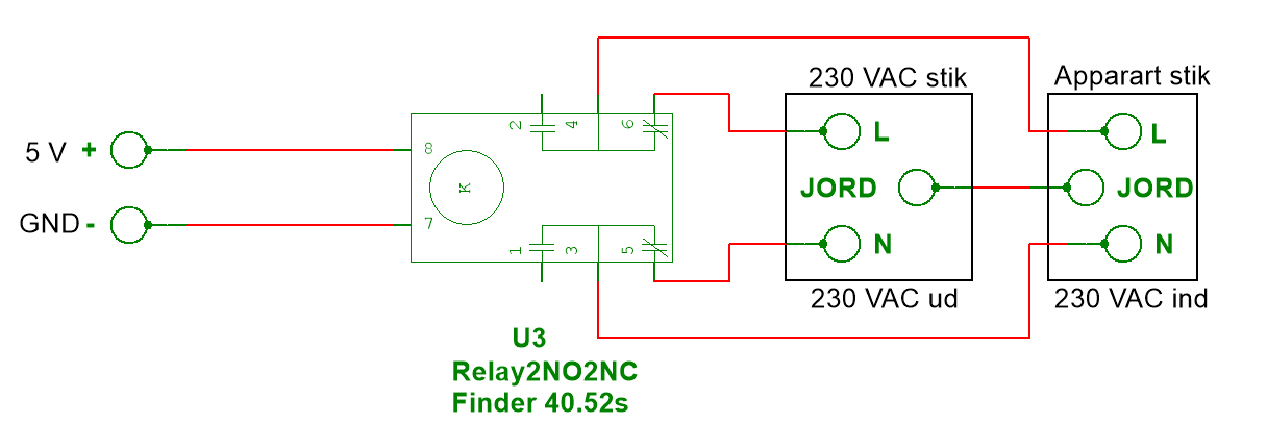
\includegraphics[width=0.75\textwidth]{Billeder/230VAC_KREDS}
    \caption{Kredsløbsdiagram for lukket 230 V / 5 V relæ}
    \label{lab:Relay_box}
\end{figure}

\subsubsection{Relæ styring}

PSoC4 giver ikke nok spænding eller strøm til sprinkler relæet, det har derfor været nødvendigt at føre signalet igennem en transistor som det ses på figur \ref{lab:BC517}. Relæet kræver en strøm på 100 mA og den trækker indenfor 3,7 V -8,8 V, dette problem løser BC517 transistoren. 

\begin{figure}[H] \centering
{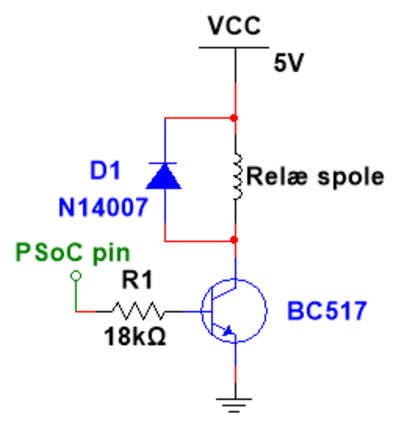
\includegraphics[width=0.3\textwidth]{Billeder/BC517}}
\caption{BC517 opsætning}
\label{lab:BC517}
\raggedright
\end{figure} 

Modstanden R1 er indsat for at begrænse den strøm der går ind i transistorens base ben, ifølge databladet må base benet højst belastet med 100 mA. Ibase strømmen er beregnet ud fra Ohms lov og der er valgt en modstand på 18 kohm, der begrænser strømmen til 0,1 mA, se formel \ref{eq:Ibase}.

\begin{equation} 
Ibase = \frac{3,3V - 1,4V}{18k\Omega} = 0,1mA
\label{eq:Ibase}
\end{equation} 

Når PSoC4’s pin til BC517 transistoren går høj (3,3V), så skabes der forbindelse mellem collector og emitter på transistoren, herved er der spænding over relæets spole og relæets kontaktsæt klikker herved. Yderlige overvejelser og information kan findes i projektdokumentation afsnit 5.4.3, Relæ-styring.




